%%%%%%%%%%%%%%%%%%%%%%%%%%%%%%%%%%%%%%%%%%%%%%%%%%%%%%%%%%%%%%%%%%%%%
%
%  This is a sample LaTeX input file for your contribution to 
%  the M&C2019 topical meeting.
%
%  Please use it as a template for your full paper 
%    Accompanying/related file(s) include: 
%       1. Document class/format file: mandc.cls
%       2. Sample Postscript Figure:   figure.pdf
%       3. A PDF file showing the desired appearance: mandc2019_template.pdf
%       4. cites.sty and citesort.sty that might be needed by some users 
%    Direct questions about these files to: palmert@engr.orst.edu
%											mark.dehart@inl.gov
%
%    Notes: 
%      (1) You can use the "dvips" utility to convert .dvi 
%          files to PostScript.  Then, use either Acrobat 
%          Distiller or "ps2pdf" to convert to PDF format. 
%      (2) Different versions of LaTeX have been observed to 
%          shift the page down, causing improper margins.
%          If this occurs, adjust the "topmargin" value in the
%          physor2018.cls file to achieve the proper margins. 
%
%%%%%%%%%%%%%%%%%%%%%%%%%%%%%%%%%%%%%%%%%%%%%%%%%%%%%%%%%%%%%%%%%%%%%


%%%%%%%%%%%%%%%%%%%%%%%%%%%%%%%%%%%%%%%%%%%%%%%%%%%%%%%%%%%%%%%%%%%%%
\documentclass[letterpaper]{mandc2019}
%
%  various packages that you may wish to activate for usage 
\usepackage{tabls}
\usepackage{cites}
\usepackage{epsf}
\usepackage{appendix}
\usepackage{ragged2e}
\usepackage[top=1in, bottom=1.in, left=1.in, right=1.in]{geometry}
\usepackage{enumitem}
\setlist[itemize]{leftmargin=*}
\usepackage{caption}
\captionsetup{width=1.0\textwidth,font={bf,normalsize},skip=0.3cm,within=none,justification=centering}
\usepackage{float}
\usepackage{algorithm}
\usepackage{algorithmic}
\usepackage{subcaption}

%\usepackage[justification=centering]{caption}

%
% Define title...
%
\title{APPROACHES TO LOAD BALANCING \\
MASSIVELY PARALLEL TRANSPORT SWEEPS \\
 ON UNSTRUCTURED GRIDS}
%
% ...and authors
%
\author{%
  % FIRST AUTHORS 
  %
  \textbf{Tarek Habib Ghaddar$^1$, Jean C. Ragusa$^1$}%\footnote{Footnote, if necessary, in Times New Roman font and font size 10} \\
  $^1$Dept. of Nuclear Engineering, Texas  A\&M University \\
  College Station, TX, 77843-3133 \\ 
\\
  \url{tghaddar@tamu.edu}, \url{jean.ragusa@tamu.edu}
}
%
% Insert authors' names and short version of title in lines below
%
\newcommand{\authorHead}      % Author's names here use et al. if more than 3
           {First author}  
\newcommand{\shortTitle}      % Short title here (Shorten to fit all into a single line)
           {Paper Title }  
%%%%%%%%%%%%%%%%%%%%%%%%%%%%%%%%%%%%%%%%%%%%%%%%%%%%%%%%%%%%%%%%%%%%%
%
%   BEGIN DOCUMENT
%
%%%%%%%%%%%%%%%%%%%%%%%%%%%%%%%%%%%%%%%%%%%%%%%%%%%%%%%%%%%%%%%%%%%%%
\begin{document}
\maketitle
\justify 

\section{INTRODUCTION} 
When discussing the parallel scaling of transport sweeps, a load balanced problem is of great importance. A load balanced problem has an equal number of degrees of freedom per processor. Load balancing is important in order to minimize idle time for all processors by equally distributing (as much as possible) the work each processor has to do.  For the purposes of unstructured meshes in PDT, Texas A\&M's massively parallel radiation transport code, we are looking to ``balance'' the number of cells. Ideally, each processor will be responsible for an equal number of cells. 

\section{UNSTRUCTURED MESHES IN PDT} 
\label{sec:first}

In order to understand how load balancing is handled in PDT, we first describe the the partitioning scheme and how the mesh is distributed amongst processes.  In general:
\vspace{-1cm}
\begin{itemize}\itemsep 1pt \parskip 0pt \parsep 0pt
\item ``Cut lines" (planes for 3D) are used to slice through the mesh in the x,y, and z dimensions.
\item The cut planes form brick partitions, called subsets, that have unstructured meshes inside of them. 
\item The subsets are distributed amongst the processor domain.
\end{itemize}
\vspace{-1cm}

Both approaches to load balancing discussed in this paper rely on the concept of a subset. Figure \ref{subset_example} illustrates a 2D example of a subset, where the lower left and lower right subsets are highlighted in blue and black boxes, respectively. 

\begin{figure}[H]
\centering
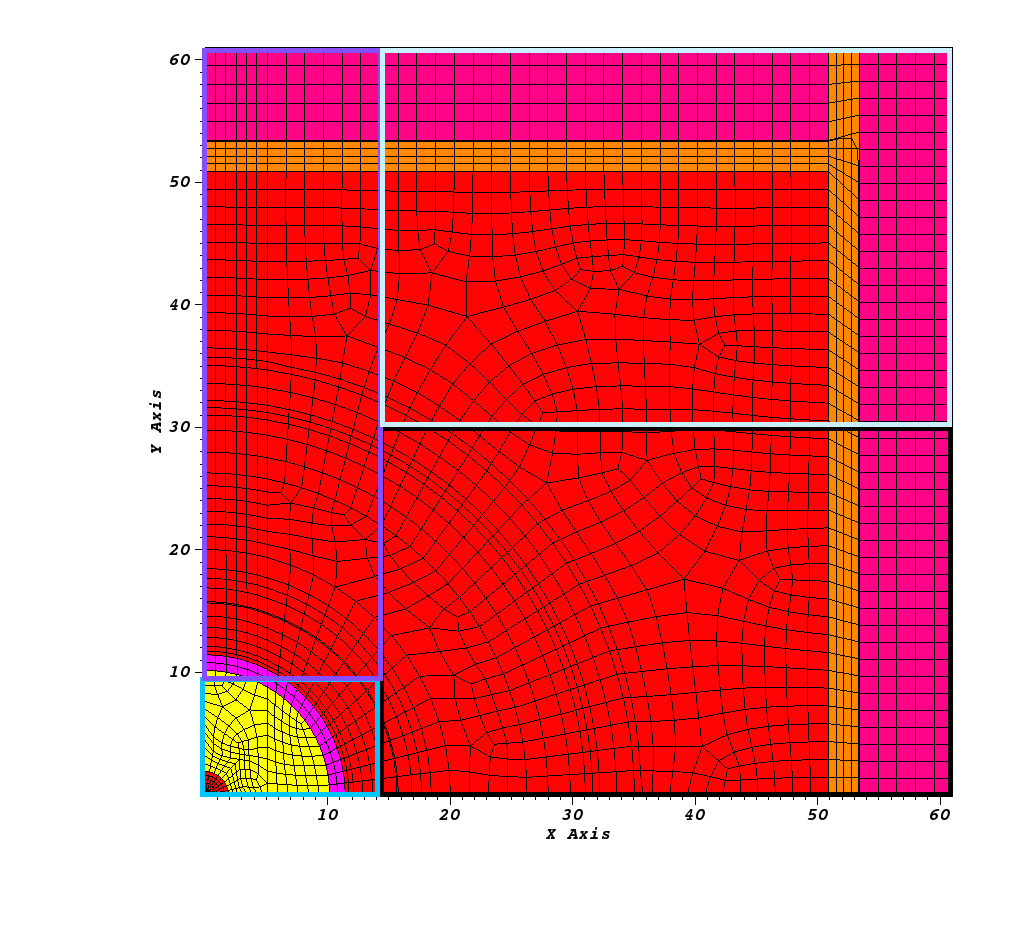
\includegraphics[scale=0.5,trim={3cm 2cm 1cm 1cm},clip]{figures/subset_example.png}
\caption{A 2D mesh partitioned into four subsets.}
\label{subset_example}
\end{figure}

\section{LOAD BALANCING IN PDT}

All approaches to load balancing in PDT rely on the movement of cut lines (or planes) to redistribute cells more evenly across all subsets. In general, this means moving cut lines into more mesh dense regions in order to better focus processing power. We first define a metric describing how imbalanced our problem is:
\begin{equation}
f =\frac{\underset{ijk}{\text{max}}(N_{ijk})}{\frac{N_{tot}}{I\cdot J\cdot K}},
\label{metric_def}
\end{equation}
where $f$ is the load balance metric, $N_{ijk}$ is the number of cells in subset $(i,j,k)$, $N_{tot}$ is the global number of cells in the problem, and $I$, $J$, and $K$ are the total number of subsets in the $x$, $y$, and $z$ direction, respectively. The metric is a measure of the maximum number of cells per subset divided by the average number of cells per subset.

The load balancing algorithm moves cut planes based on dimensional sub-metrics, $f_d$ . Equation ~\eqref{submetric} defines these two parameters:
\begin{equation}
f_{D} = \underset{d}{\text{max}}[\sum_{d2,d3} N_{ijk}]/\frac{N_{tot}}{D}
\label{submetric}
\end{equation}
$f_{d}$ is calculated by taking the maximum number of cells per row, column, or plane and dividing it by the average number of cells per the corresponding dimension. If this number is greater than predefined tolerances, the cut lines in the respective dimension is redistributed. Once redistribution occurs, a new metric is calculated. This iterative process occurs until a maximum number of iterations is reached, or until $f$ converges within the user defined tolerance. In general, our approaches to load balancing follow this simple algorithm:

\begin{algorithm}
\begin{algorithmic}

\WHILE {$f > \text{tol}_{\text{subset}}$}
\FOR{d in $x,y,z$}
	\IF {$f_D> \text{tolerance}_{d}$}
		\STATE Redistribute cut lines corresponding to dimension d.
	\ENDIF	
\ENDFOR
\ENDWHILE
\end{algorithmic}
\end{algorithm}

Our initial approach to load balancing involved placing cut lines in all dimensions all the way through the mesh. This created an orthogonal partitioning where each subset had an equivalent number of neighbors. This was done to preserve the optimal sweep partitioning described by Adams et. al \cite{mpadams2015}. However, there are theoretical limits to load balancing in this fashion. Figure \ref{2dgeneral} shows a simple 2D subset layout with $M$ unaligned patches of high mesh density.

\begin{figure}[H]
\centering
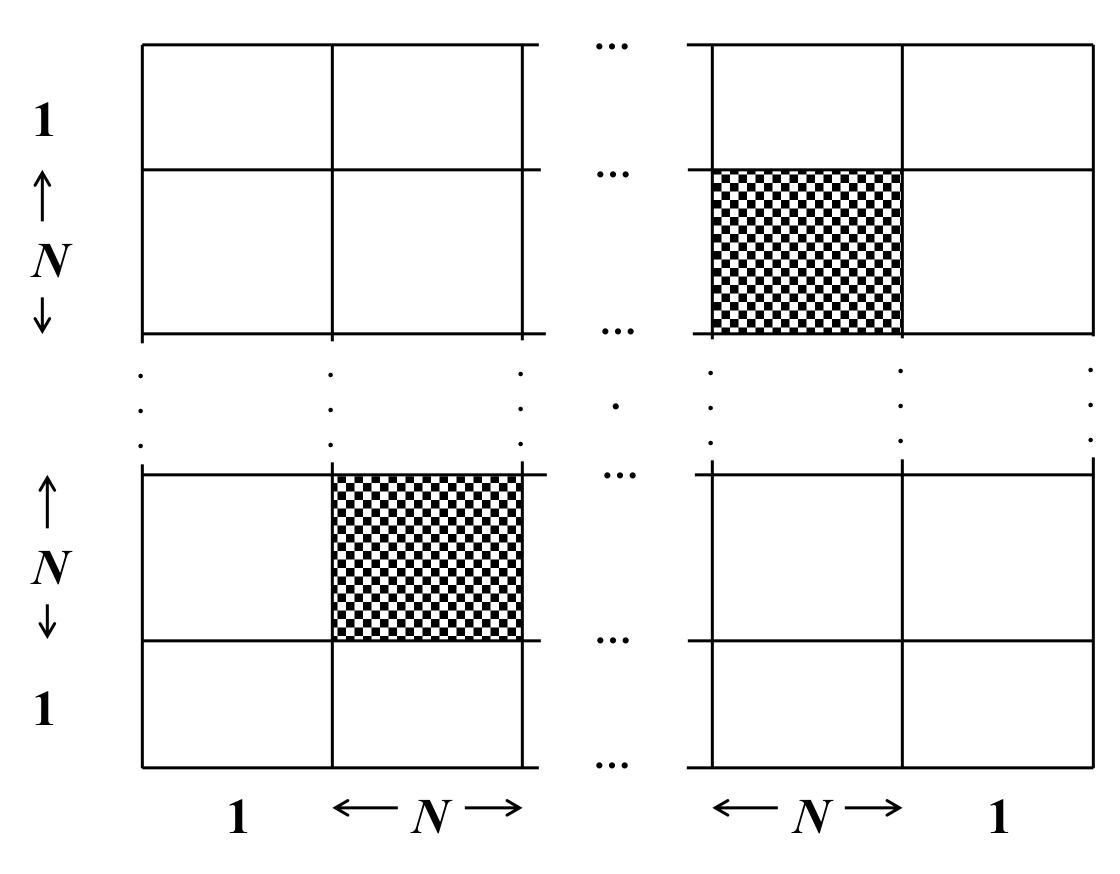
\includegraphics[scale=0.6]{figures/2dgeneral.png}
\caption{A 2D subset layout with $M$ unaligned patches of high mesh density.}
\label{2dgeneral}
\end{figure}

The subset layout is $[M(N+1)+1] \times [M(N+1)+1]$, but only $MN^2$ subset have significant work, leading to a theoretical limit for the load imbalance factor:
\begin{equation}
f= \frac{\left( M(N+1)+1 \right)^2}{MN^2} \xrightarrow{N\to \infty} \frac{M^2N^2}{MN^2} = M.
\end{equation}

An improved load balancing algorithm was implemented that significantly improved our metric. Rather than load balancing both dimensions within an iteration, one dimension is balanced first for all iterations, and then the cut lines that yielded the best metric for that dimension are chosen. Then the next dimension is balanced within the first dimension. For example, if the $x$ cut lines are balanced first, the $y$ cut lines would be balanced \textit{within} each column. When full 3D load balancing by dimension, shown in Fig. \ref{lbd}, excellent metrics within 5\% of unity are consistently obtained.

\begin{figure}[H]
\centering
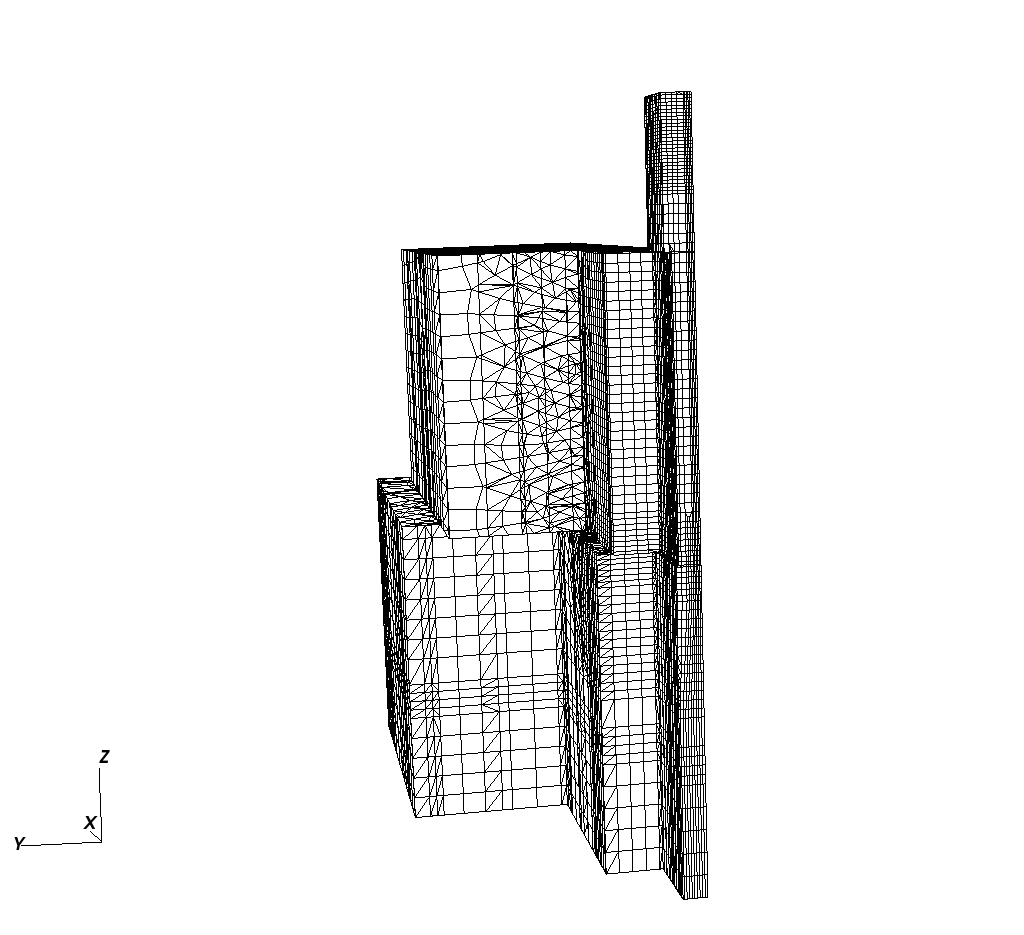
\includegraphics[scale=0.5]{figures/im1_foam_448.png}
\caption{A slice of the IM1C experiment showcasing load balancing by dimension in 3D.}
\label{lbd}
\end{figure}

The full paper will be showing scaling results obtained using load balanced meshes.

\section{CONCLUSIONS AND FUTURE WORK}

While we obtain excellent imbalance factors utilizing the load balance by dimension algorithm (particularly for 3D cases), further study shows the possibility that the most efficient partitioning scheme is not being used. 
While perfect load balance was the initial goal, we need to know how this affects the efficiency of our parallel transport sweep. Figures \ref{regular_partition}-\ref{worst_partition} showcase the theoretical effect of perfect load balance on the transport sweep.

Figure \ref{regular_partition} shows a sweep domain with a regular partition with perfect balance (equivalent number of cells per processor). The sweep maintains a mostly regular wavelike structure as each angle sweeps through the domain, and this sweep completes in 40 stages. This is the ideal partitioning for the transport sweep, but often hard to achieve with unstructured meshes \textbf{and} perfect balance.

\begin{figure}[H]
  \centering
  \begin{subfigure}{0.49\textwidth}
  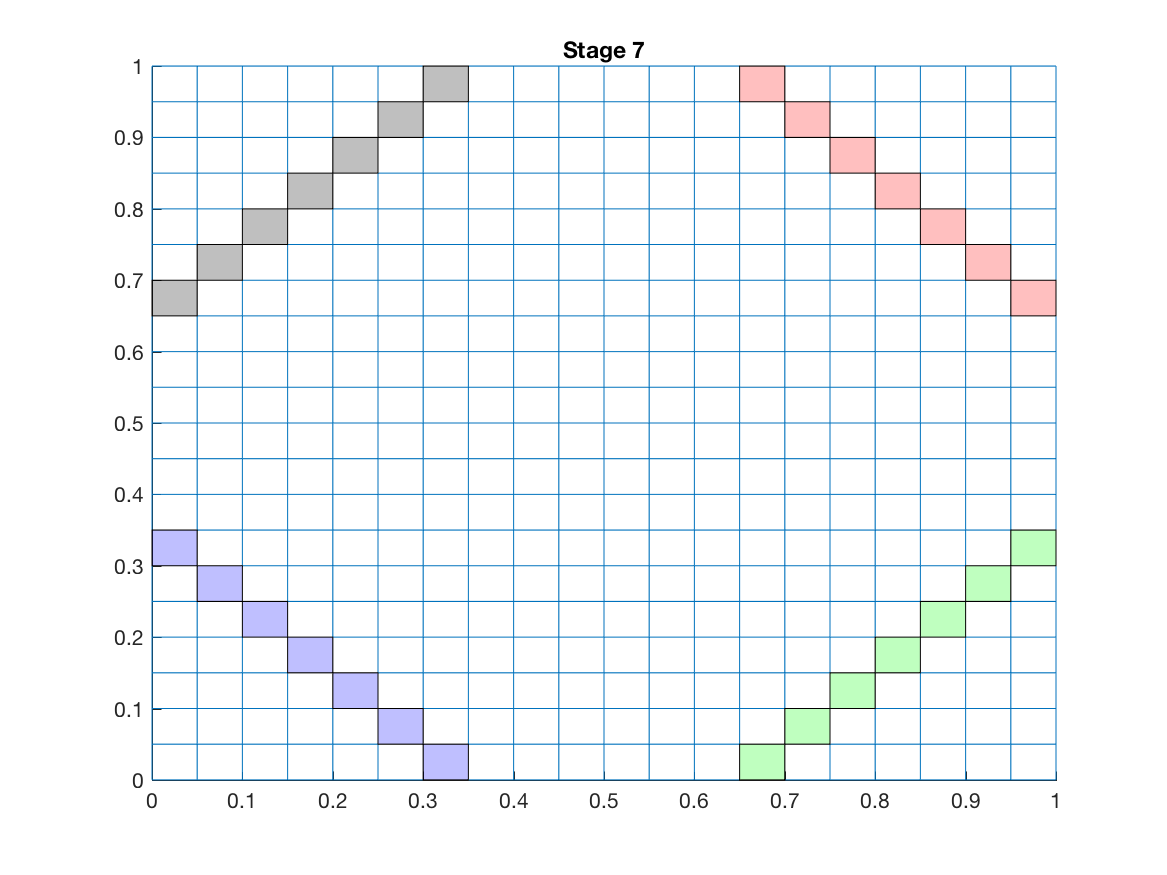
\includegraphics[scale=0.5]{figures/regular_partition_1.png}
  \end{subfigure}
  \begin{subfigure}{0.49\textwidth}
  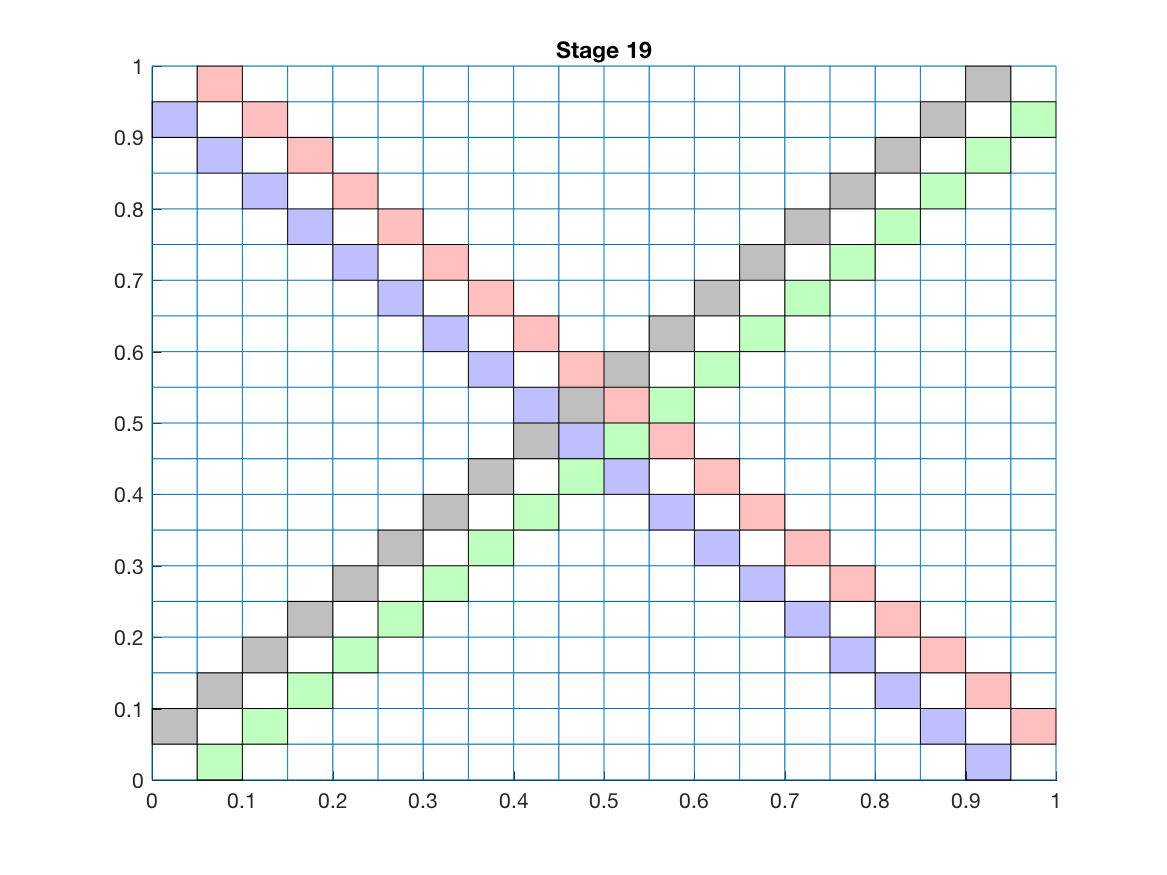
\includegraphics[scale=0.5]{figures/regular_partition_2.png}
  \end{subfigure}
  \begin{subfigure}{0.49\textwidth}
  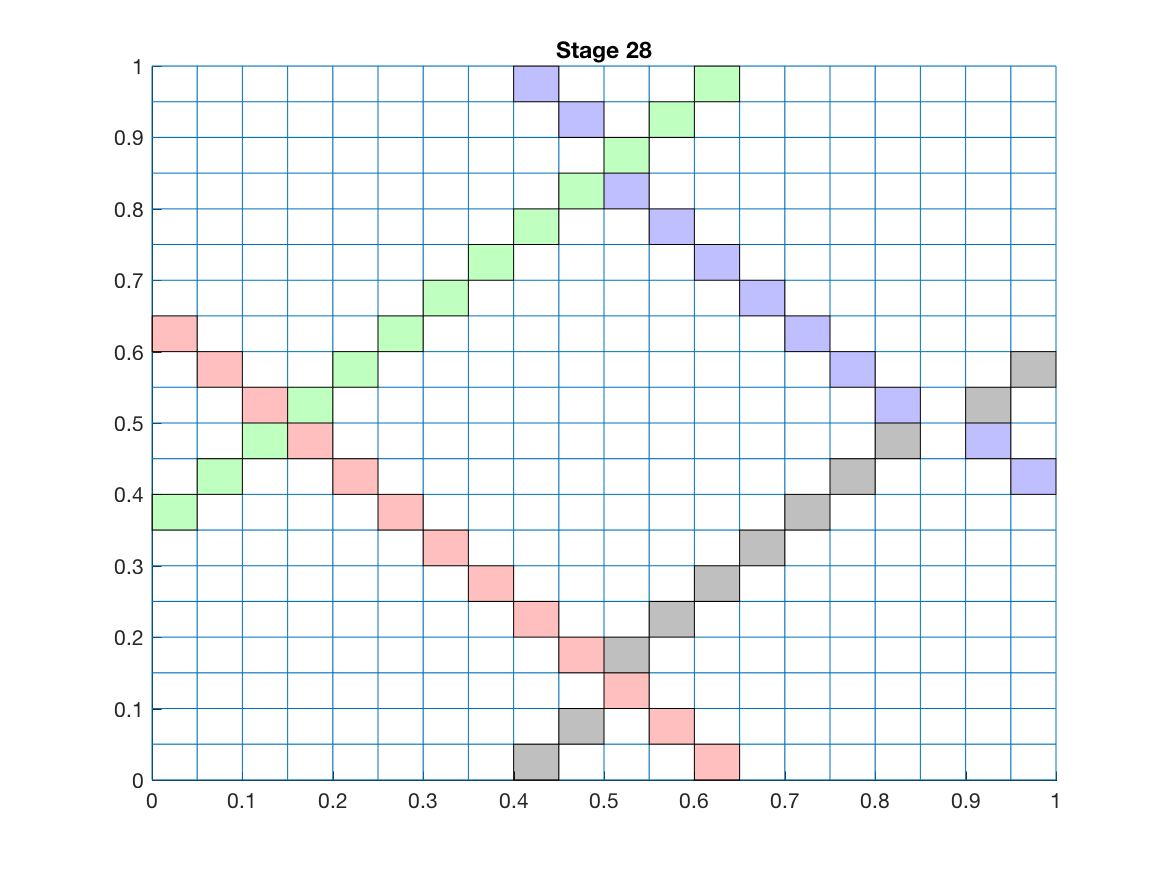
\includegraphics[scale=0.5]{figures/regular_partition_3.png}
  \end{subfigure}
  \begin{subfigure}{0.49\textwidth}
  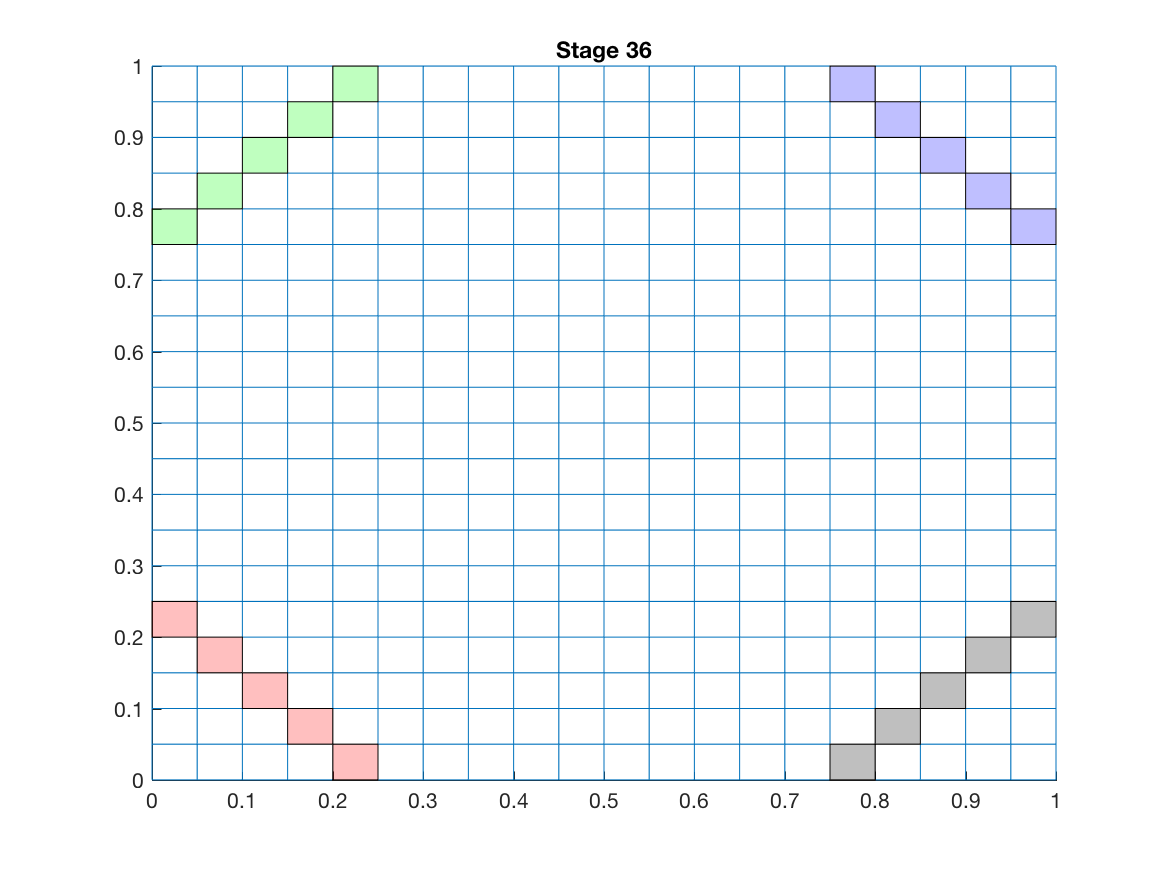
\includegraphics[scale=0.5]{figures/regular_partition_4.png}
  \end{subfigure}
  \caption{The transport sweep using a regular partition with perfect balance.}
  \label{regular_partition}
\end{figure}

With the improved load balancing by dimension, we are likely to see a partition similar to the partitioning shown in Fig. \ref{random_partition} for all geometries. It is immediately observable that we don't have the same wavelike transport sweep, as communication penalties take their toll. As a result, this sweep completes in 101 stages, as opposed to 40 stages for the regular partition.


\begin{figure}[H]
  \centering
  \begin{subfigure}{0.49\textwidth}
  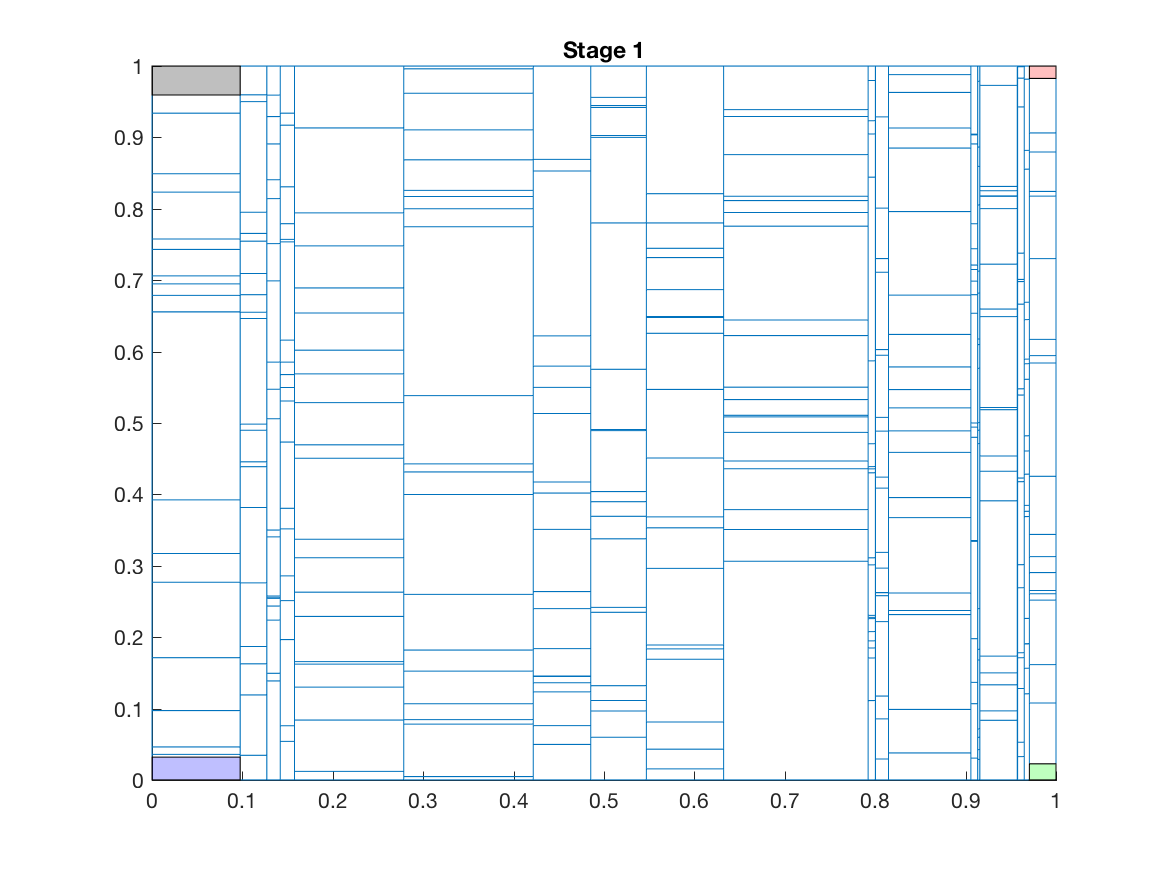
\includegraphics[scale=0.5]{figures/random_partition_1.png}
  \end{subfigure}
  \begin{subfigure}{0.49\textwidth}
  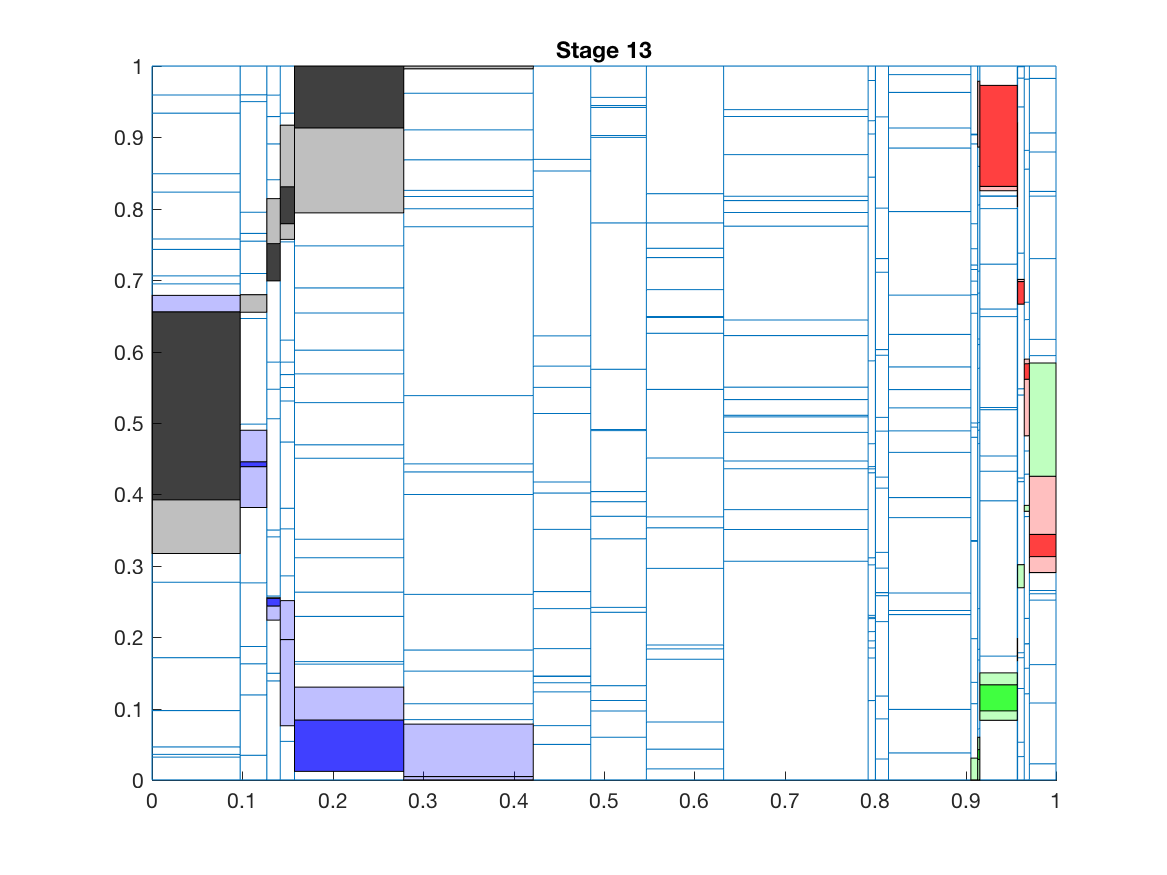
\includegraphics[scale=0.5]{figures/random_partition_2.png}
  \end{subfigure}
  \begin{subfigure}{0.49\textwidth}
  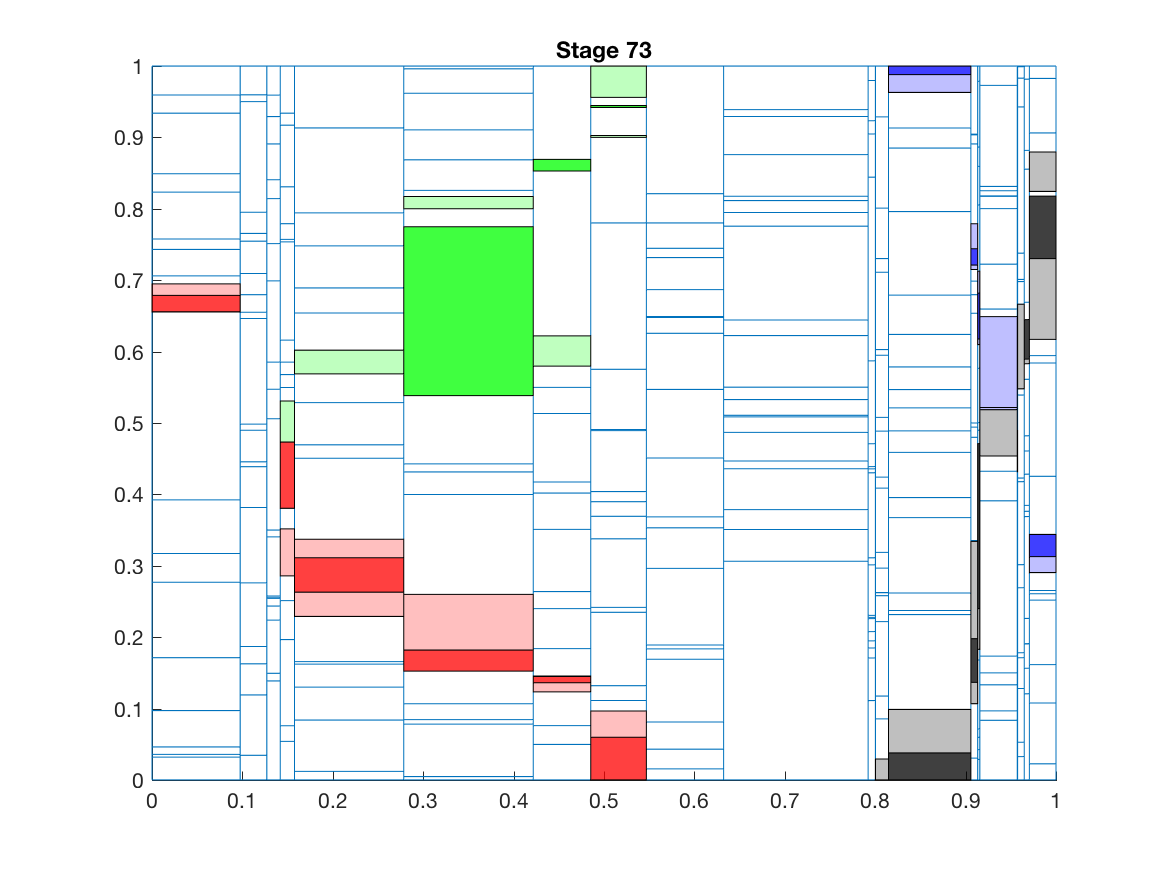
\includegraphics[scale=0.5]{figures/random_partition_3.png}
  \end{subfigure}
  \begin{subfigure}{0.49\textwidth}
  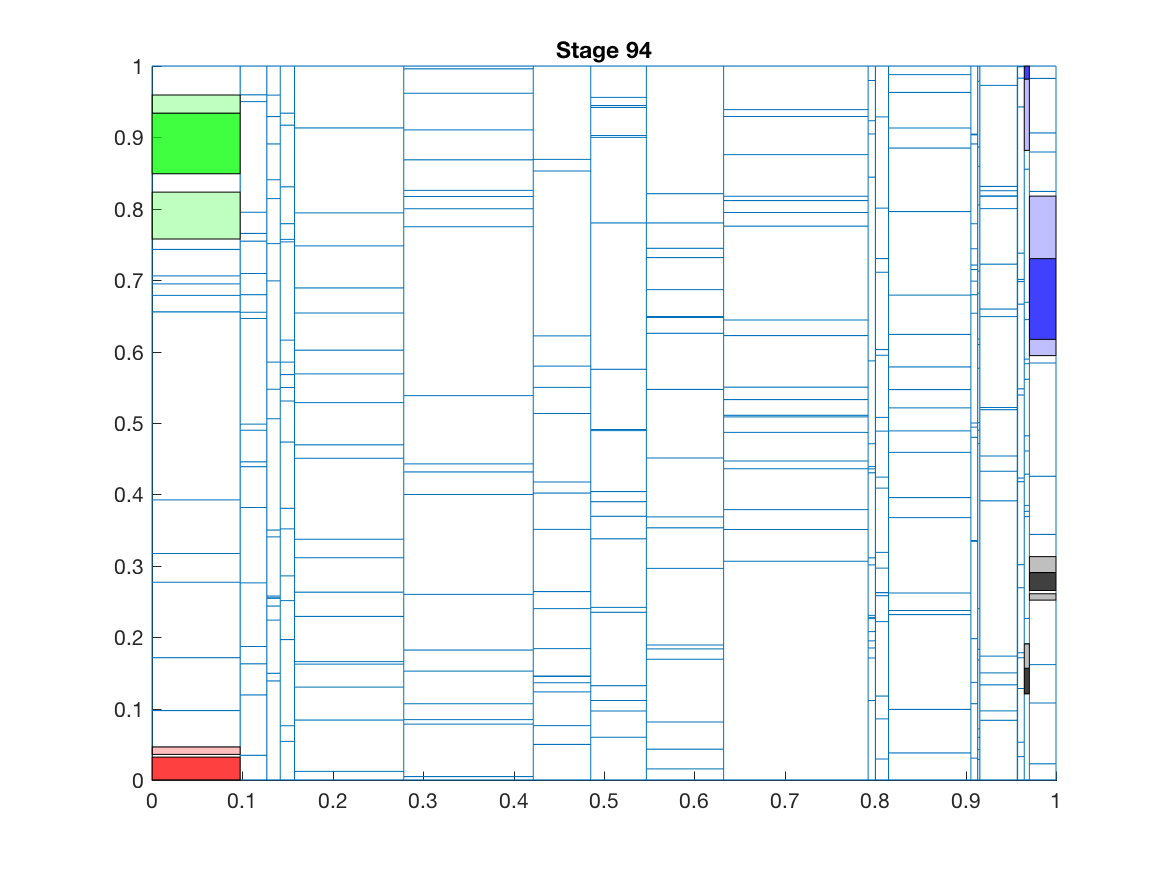
\includegraphics[scale=0.5]{figures/random_partition_4.png}
  \end{subfigure}
  \caption{The transport sweep using a random partition with perfect balance.}
  \label{random_partition}
\end{figure}

Figure \ref{worst_partition} observes the worst theoretical sweep partitioning, where the transport sweep takes on a snake-like behavior. This partitioning yields a stage count of 230, which is far worse than even the random partitioning stage count of 101.

\begin{figure}[H]
  \centering
  \begin{subfigure}{0.49\textwidth}
  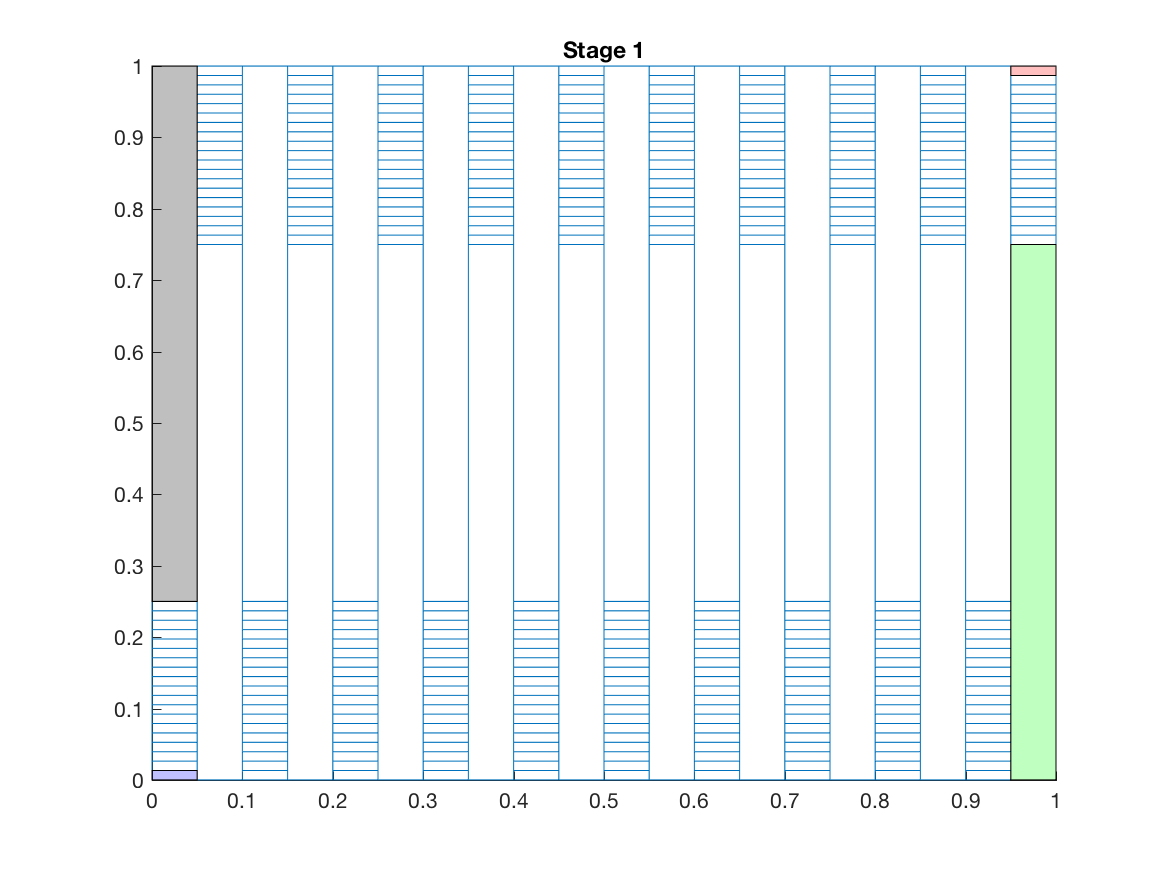
\includegraphics[scale=0.5]{figures/worst_partition_1.png}
  \end{subfigure}
  \begin{subfigure}{0.49\textwidth}
  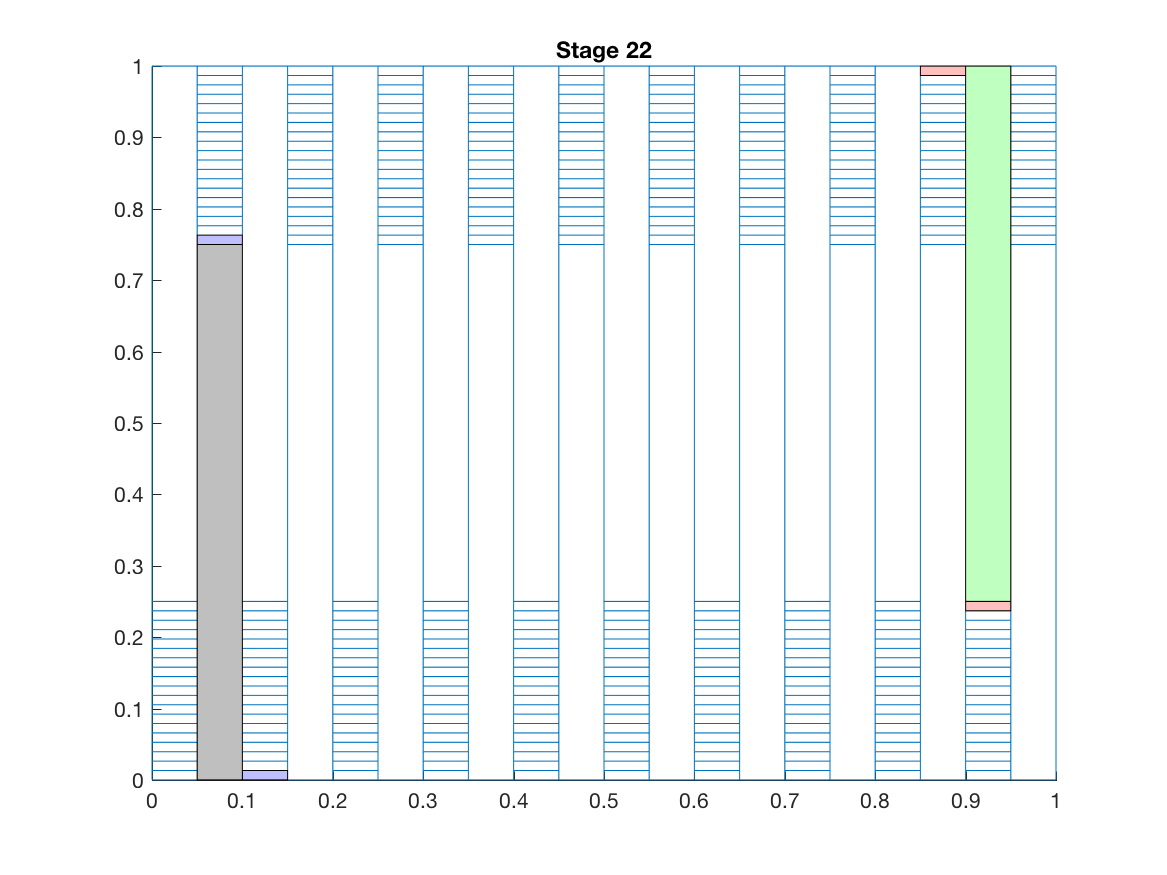
\includegraphics[scale=0.5]{figures/worst_partition_2.png}
  \end{subfigure}
  \begin{subfigure}{0.49\textwidth}
  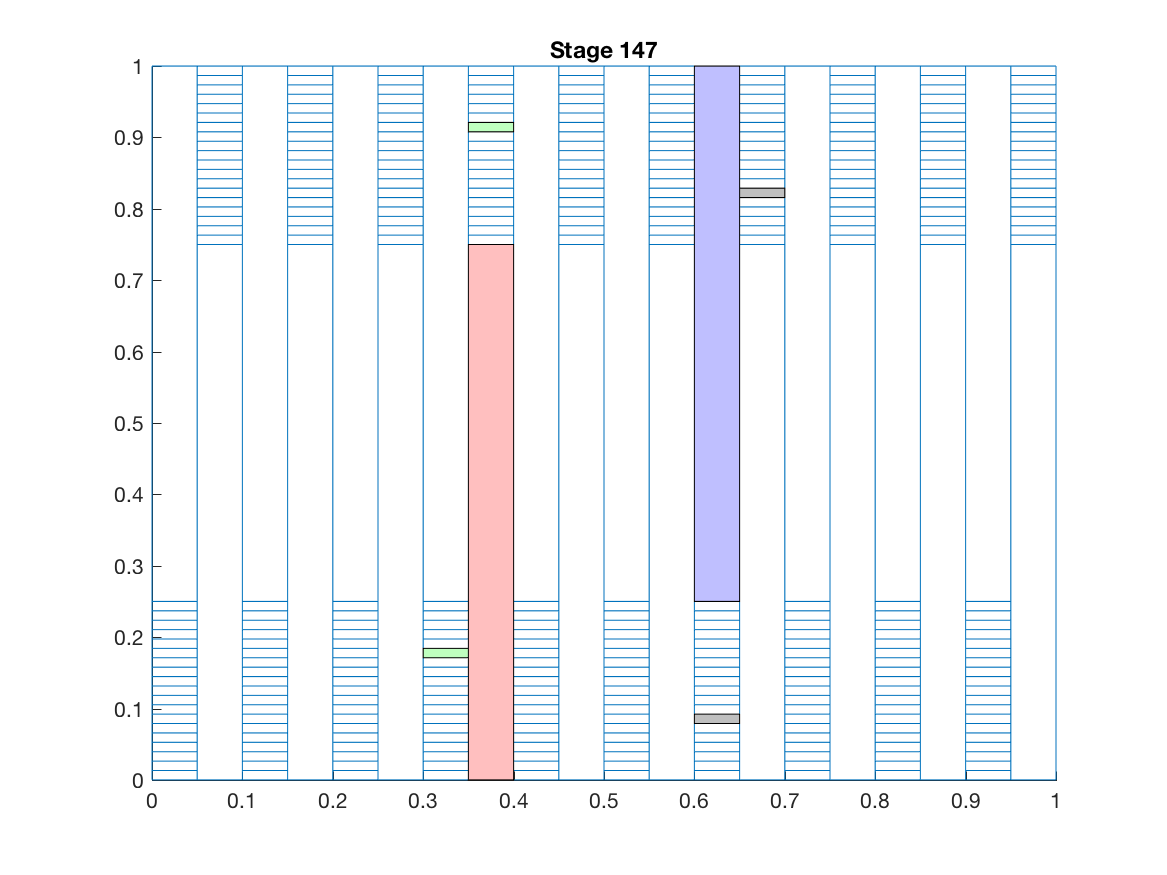
\includegraphics[scale=0.5]{figures/worst_partition_3.png}
  \end{subfigure}
  \begin{subfigure}{0.49\textwidth}
  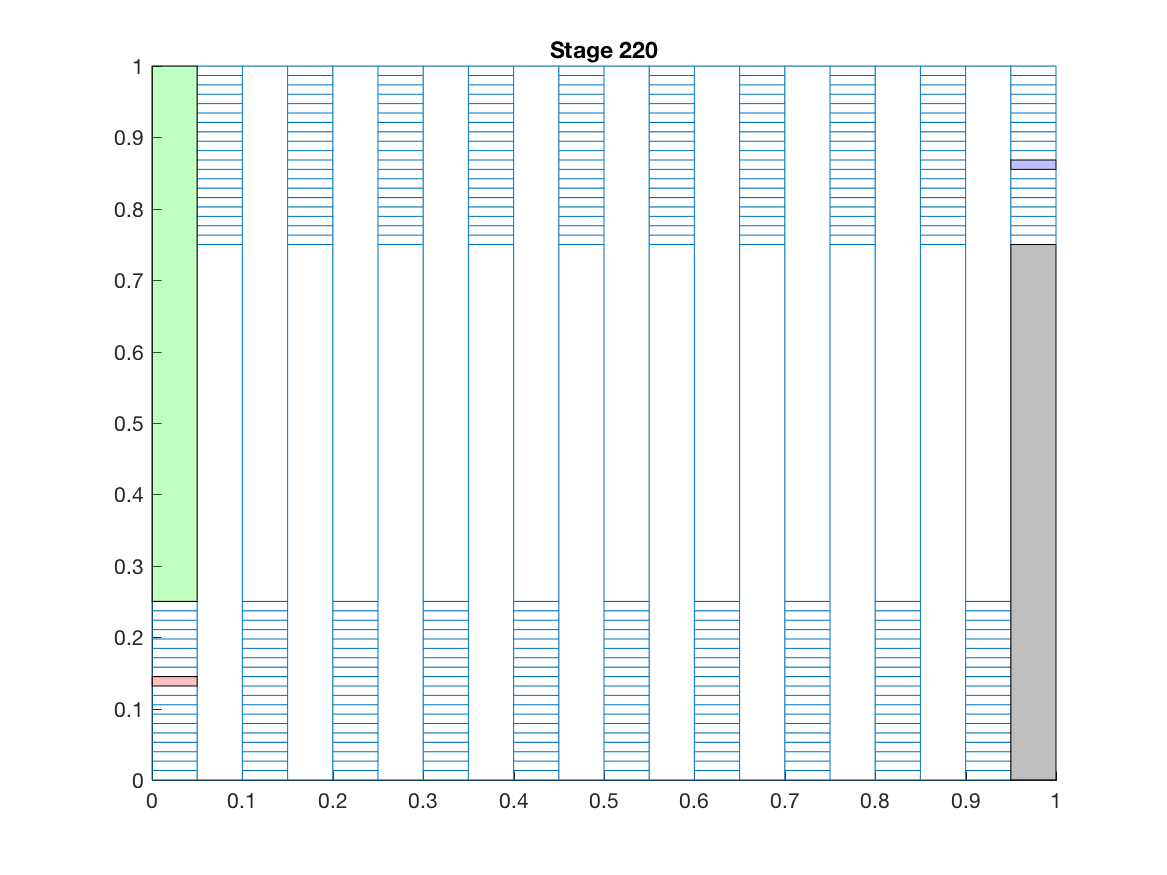
\includegraphics[scale=0.5]{figures/worst_partition_4.png}
  \end{subfigure}
  \caption{The transport sweep using the worst partition with perfect balance.}
  \label{worst_partition}
\end{figure}

Future studies and research will attempt to find an optimal partitioning scheme that both takes into account load balancing as well as partitioning for the transport sweep.

% You can enter a bibliography into the document using the following format, or use the 
% bibliography style file "mandc.bst" found in the template directory.  You can use the bibliography style file
% by replacing the current bibliography block with:
 \setlength{\baselineskip}{12pt}
 \bibliographystyle{mandc}
 \bibliography{mandc}


\end{document}
